\section{Methodology}
To understand the flow behaviour in various undertray geometry, fluid dynamics analysis is required. The rapid development of computational power has allowed more accurate and reliable computational analysis results such as computational fluid dynamics (CFD) \cite{Andersson2011ComputationalEngineers}. The usage of CFD allows engineers to simplify the processes and achieve an accurate result in a more abbreviated time, allowing engineers to do more iterations. 

\begin{figure}[!htb]
    \centering
    \makebox[\textwidth]{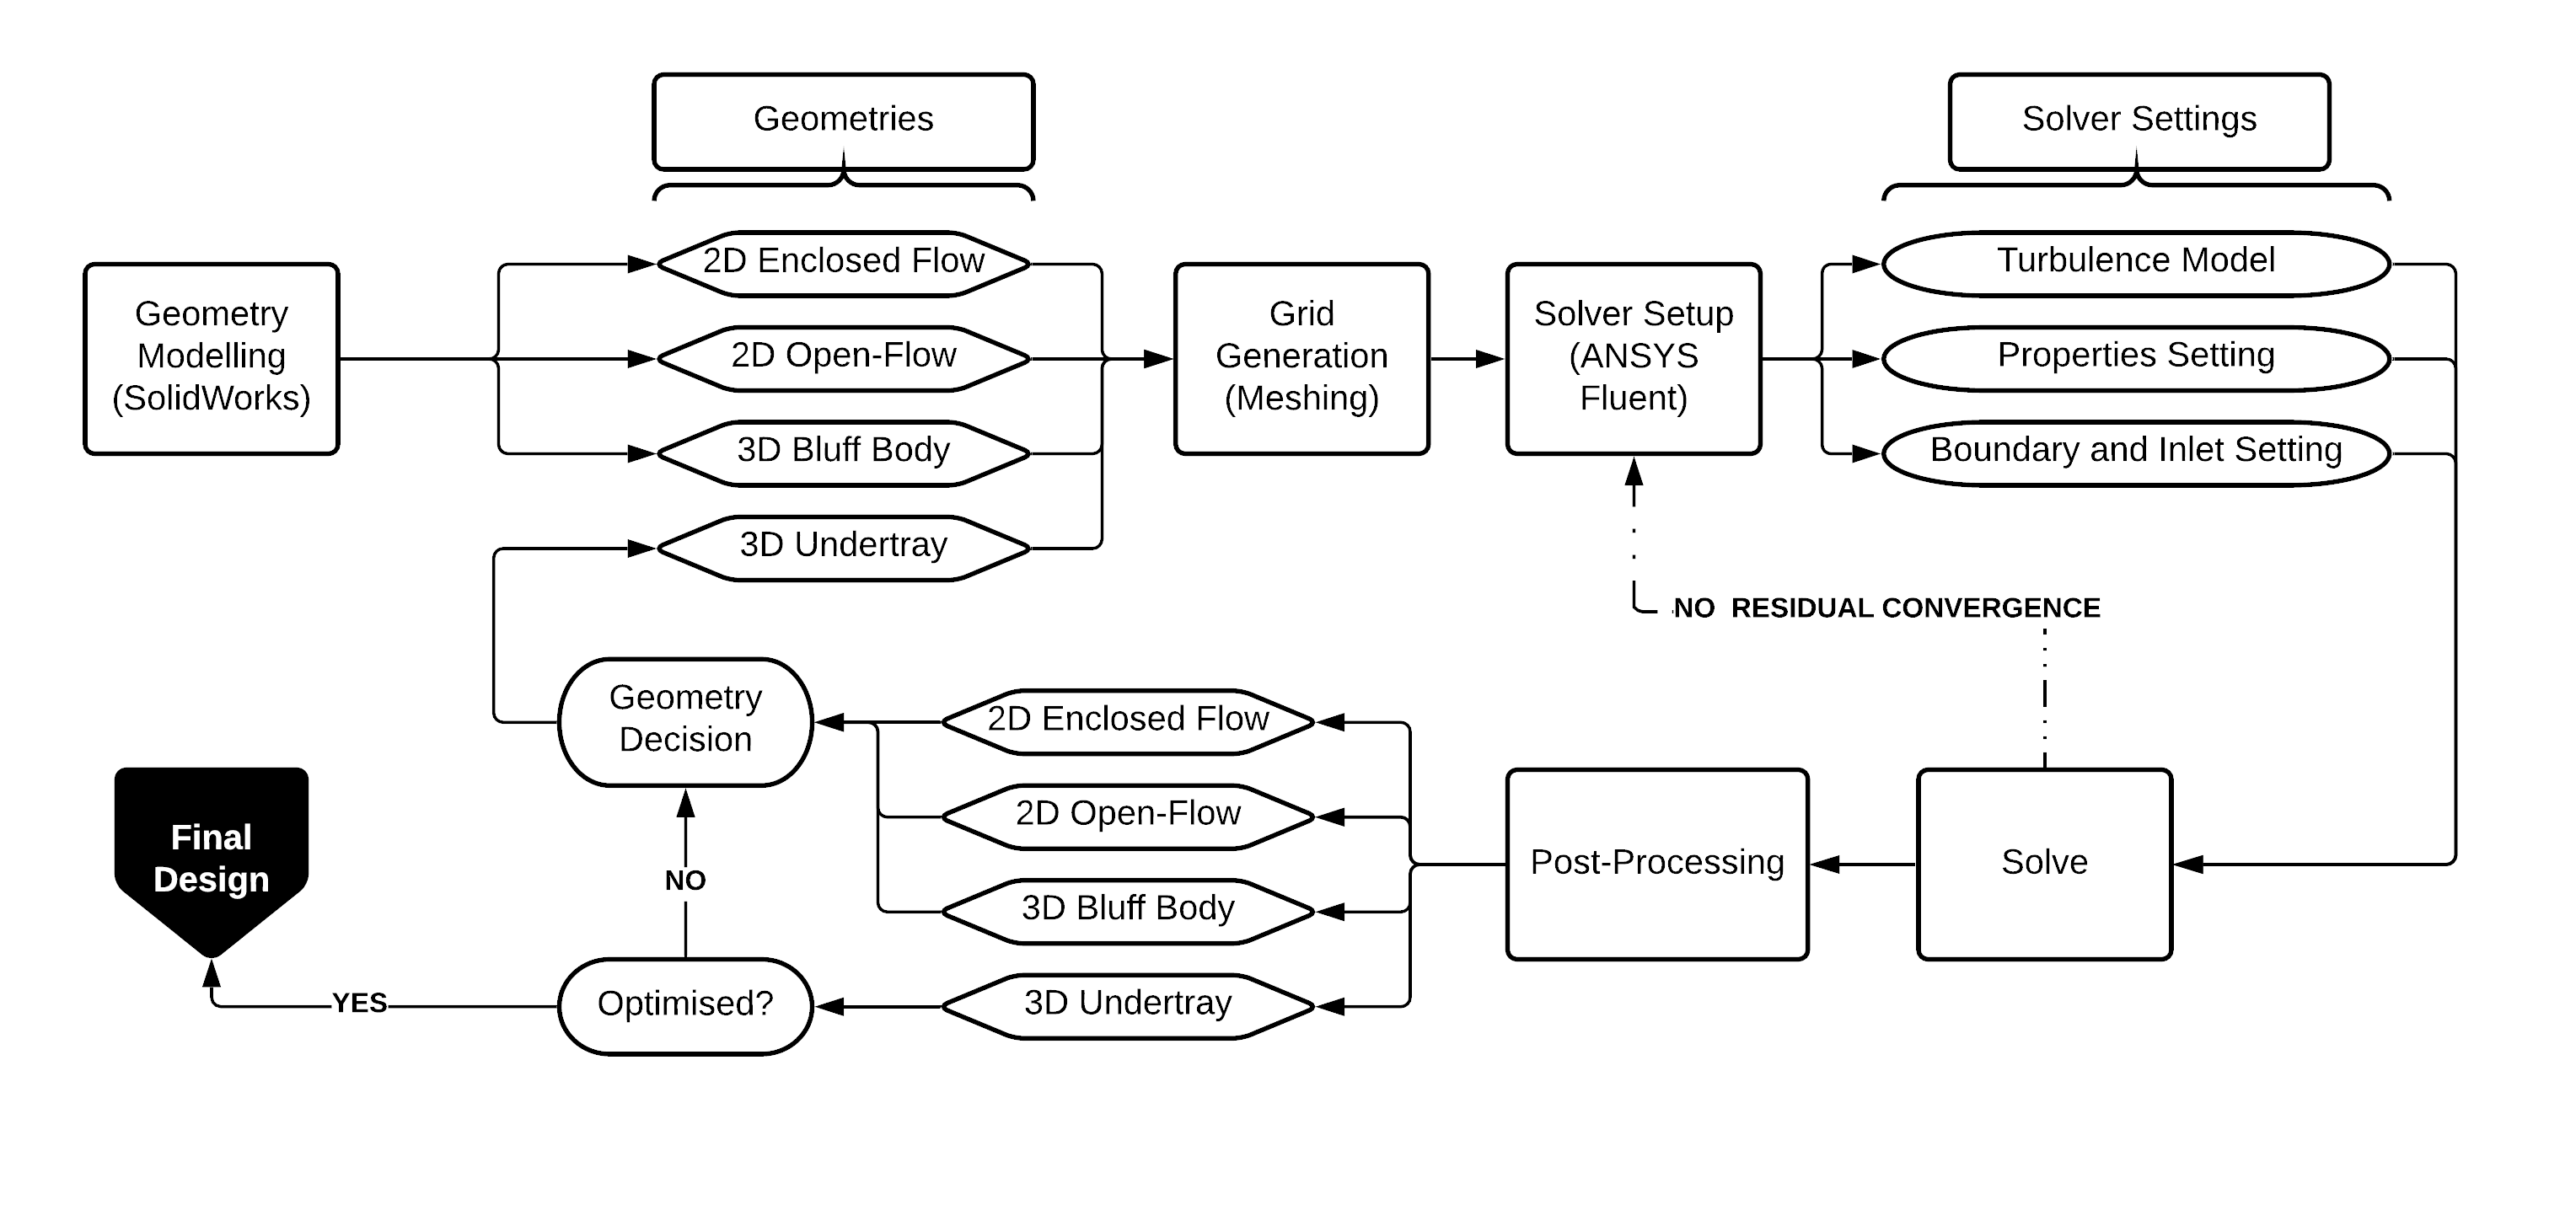
\includegraphics[scale=0.15]{Figures/project_methodology_chart.png}}
    \caption{Project Methodology Flow Chart}
    \label{fig:project methodology}
\end{figure}

\noindent The methodology consists of 3 phase, which are 2D enclosed \& open-flow, 3D bluff body, 3D undertray. The first phase is the 2D analysis, which analyses the undertray variables on a Venturi-tube like geometry and open-flow analysis to analyse a simple bluff body with similar undertray variables. The 3D bluff body will take the 2D geometry, extrude it as a 3D geometry, and then analyse it with the identical undertray variables. Lastly is the 3D undertray, where the optimised results from previous analysis will be used to determine the final undertray design's geometry. A simplified traced body from the QFR 2021 car will be attached to the undertray to achieve pragmatic results. The process flow can be illustrated in figure \ref{fig:project methodology}. This paper will be entirely based on CFD, which utilises ANSYS Fluent as a default working platform.

\subsection{Pre-Processing \& Solver Setup}

\subsubsection{Grid Generation (Meshing)}
\noindent The surface or body which have been defined from SolidWorks becomes the basis for the meshing. The meshing app, which integrated with ANSYS Workbench, provide a user-friendly, simple, and fast meshing generator. Due to the constrain of computational power and time, unstructured triangular (2D) and tetrahedral (3D) mesh were widely used with a quadrilateral (2D) and triangular prism (3D) near the wall as an inflation layer to capture the growth of the boundary layer and reduce numerical diffusion \cite{Lanfrit2005BestFLUENT}.

\noindent Looking back to the 2D and 3D bluff body simulation goal is to obtain and analyse the trend in geometry changes of an undertray; therefore, a non-detailed yet decent mesh could be generated. Local refinement around the body that affected by the fluid flow is recommended \cite{Lanfrit2005BestFLUENT} to achieve reasonable results and flow representation, especially around the undertray; moreover, this technique allows larger mesh on the far-field section less likely to be affected or affecting the result. Another aspect of reasonable meshing is to be aware of the mesh properties such as skewness and growth ratio. For automotive application, it is recommended to have skewness less than 0.45 and a maximum growth rate of less than 20\% \cite{Lanfrit2005BestFLUENT}. 

\noindent One crucial facet of an undertray flow is the generation of the boundary layer and how it interacts with the moving floor, the accuracy of this aspect is dependent on the quality of layer grid growth near the wall or wall function. To generate a good inflation layer, it is essential to make sure the y+ value (first layer height grid) does not exceed the inner boundary layer region, which can be calculated using this expression:

\begin{equation}
    y^+ = \frac{\rho U_\tau \partial y}{\mu}, where \quad U_\tau = \sqrt{\frac{\tau_w}{\rho}} = U \sqrt{\frac{1}{2}C_f}
\end{equation}

\noindent Figure \ref{fig:inflation layer} shows the illustration of y$^+$  value on a wall function. The turbulence model on the solver also has to be considered in defining the y$^+$  value, some turbulence modelling requires a very low n y+, and some can tolerate a high y+ value. The detail of y$^+$ value in the various turbulent model will be discussed in the next section. 

\begin{figure}[!ht]
    \centering
    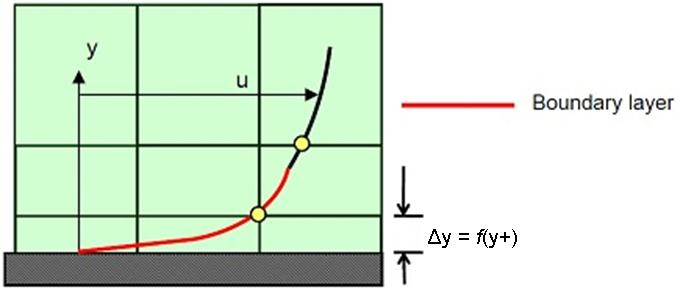
\includegraphics[height=4cm]{Figures/inflation_layer.jpg}
    \caption{Representation of grid y+ on a near wall function \cite{Anonymous2013Inflate4Blog}.}
    \label{fig:inflation layer}
\end{figure}


\subsection{Numerical Method}
\noindent The turbulence model is a crucial aspect in approximating the unsteady turbulent fluctuation \cite{Cummings2015AppliedAerodynamics}. The quality of the turbulence modelling significantly impact the fidelity of the simulations \cite{Lanfrit2005BestFLUENT}. Due to the time constraint, a variable amount, and computational power, a steady-state method was used entirely in this paper. Two-equation Reynolds-Averaged Navier-Stokes (RANS) approach was also used to solve the time-averaged flow \cite{Cummings2015AppliedAerodynamics}. With a reasonable quality of mesh, practical lift and drag trends can be achieved, which can then be studied. Realizable K-$\epsilon$ and K-$\omega$ Shear Stress Transport (SST) were used in this paper to solve the downforce and drag of the undertray and bluff body.  

\subsubsection{Realizable K-$\epsilon$  Models}
k-$\epsilon$  turbulence model is a  two-equation transport model which specifically solve the turbulence kinetic energy (k) and dissipation rate ($\epsilon$) \cite{Andersson2011Turbulent-flowModelling}\cite{Mansour1989Near-wallModeling}\cite{Ansys2006ModelingFlows}. The standard model is robust and widely used in a broad application of engineering turbulence modelling; however, the nature of  k-$\epsilon$ family is not able to calculate some of the $\epsilon$ terms which can be anticipated using wall function. Moreover, k-$\epsilon$ does not perform well for flow with strong separation and large adverse pressure gradient, which the primary feature of an undertray's diffuser \cite{Ansys2006ModelingFlows}.  Therefore realisable k-$\epsilon$ is broadly used in this analysis. The term 'realisable' itself allows some of the mathematical satisfaction in computing the Reynolds stresses, improving its turbulent flow consistency. This specific transport model is crucial to capture important flow features of an undertray, such as flow rotation, significant adverse pressure gradient, and vortex formation.

\subsubsection{k-$\omega$ Shear Stress Transport (SST) Models}
The SST model is a 2 equation-model that combine both k-$\epsilon$ and k-$\omega$ \cite{Andersson2011Turbulent-flowModelling}\cite{Ansys2006ModelingFlows}.  k-$\epsilon$ is used in the free-stream, and k-$\omega$ is used near the boundary wall means this model took the strength of both models, allowing accurate prediction in all regions. This model performs well in the region with an adverse pressure gradient and flow separation; moreover, SST is known to have better performance compared to k-$\epsilon$ and does not require any wall function\cite{Andersson2011Turbulent-flowModelling}. However, a fine mesh ($y^+  < 5$) is required on the wall, which increases the computational cost and time, as well it could over predict turbulent flow in a large strain area \cite{Andersson2011Turbulent-flowModelling}\cite{Ansys2006ModelingFlows}. 

\subsection{Boundary Conditions}
\begin{table}[!htb]
\centering
    \caption{Boundary Conditions for 2D and 3D ANSYS Fluent setup}
    \label{tab:Boundary Conditions}
\begin{tabular}{||p{3cm}|p{3cm}|p{6cm}||}
 \hline
 \centering
 Named Region  &  Boundary Condition  & Property Details\\
 \hline \hline
 \multicolumn{3}{||c||}{General Properties} \\
 \hline
 
 Inlet & Inlet velocity & Velocity = 16.667 m/s (or 40 km/h)\\
 \hline
 Outlet & Outlet Pressure  & Gauge Pressure = 0 Pa  \\
 \hline
 Undertray (2D Enclosed)/Bluff Body & Stationary Wall & No-slip condition\\
 \hline
 Moving Floor & Moving Wall & Velocity = 16.667 m/s (or 40 km/h) in the flow direction\\
 \hline
 Enclosure &   Fluid (Air)  & Pressure = 101325 Pa
Temperature = 288.15 K
Density = 1.225 kg/m3
ISA Sea Level Condition\\
 
 \hline
 \multicolumn{3}{||c||}{3D Analyses} \\
 \hline
 
 Symmetry Body & Symmetry  & -\\
 \hline
 Symmetry Top & Symmetry  & -\\
 \hline
 Symmetry Side & Symmetry & -\\
 \hline
 
\end{tabular}
\end{table}

\noindent Table \ref{tab:Boundary Conditions} shows Boundary conditions for 2D and 3D analyses in ANSYS Fluent solver. The main goal is to simulate the flow behaviour at the bottom region of the car; therefore, a moving floor was employed in all simulation with the same magnitude and direction of the flow. The usage of moving ground (or belt in a wind tunnel) is a physically correct and best option to capture a ground effect such in an undertray \cite{Zhang2006GroundCars}\cite{Burgin1986WINDEFFECT}. The simulation environment was set and assumed to International Standard Atmospheric (ISA) condition at sea level. 
\vspace{1cm}
\noindent In 3-dimensional simulation, side, far-side, and the top surface of the flow-field were set to symmetry where fluxes and normal gradients of all variables are assumed zero \cite{ANSYS2009SymmetryConditions} as recommended by Lanfrit \cite{Lanfrit2005BestFLUENT}. Along with the moving floor, this setup was surmised to provide the best results in simulating the race car or body in an actual racing track.





